\documentclass[12pt]{article}

\usepackage[OT1]{fontenc}
\usepackage[colorlinks,citecolor=blue,urlcolor=blue]{hyperref}
\usepackage{graphicx}
\usepackage{subfig}
\usepackage{fullpage}
\usepackage{palatino}
\usepackage{mathpazo}
\usepackage{amsmath}
\usepackage{amssymb}
\usepackage{color}
\usepackage{todonotes}
\usepackage{listings}
\usepackage{tikz}

\usepackage[mmddyyyy,hhmmss]{datetime}

\definecolor{verbgray}{gray}{0.9}

\lstnewenvironment{csv}{%
  \lstset{backgroundcolor=\color{verbgray},
  frame=single,
  framerule=0pt,
  basicstyle=\ttfamily,
  columns=fullflexible}}{}

\begin{document}
\begin{center}
{\Large Practical 4: Reinforcement Learning}\\
Writeup and code due at 11:59pm on Tuesday 1 May 2018\\
\end{center}

\section*{Setup}

{\bf There is no Camelot component to this practical.}  However, your main deliverables are still largely the same: a 3-4 page PDF writeup that explains how you tackled the problems.  There are two other differences with the previous practicals: you are \textbf{not} allowed to use off-the-shelf planning/RL software, and you should {\bf turn in all of your code through GitHub with a README that explains how to run it.} As before, you will do this assignment in groups of three.  You can seek partners on Piazza.  Course staff can also help you find partners. Submit one writeup per team by the due date via Canvas.  This practical requires installing the \verb|pygame| module. You can do so by following the instructions at \url{http://www.pygame.org/wiki/GettingStarted}


\section*{Introduction}

In 2013, the mobile game \emph{Flappy Bird} took the world by storm.  After its discontinuation, iPhones with the game installed sold for thousands of dollars on eBay.  In this practical, you'll be developing a reinforcement learning agent to play a similar game, \emph{Swingy Monkey}.  See screenshot in Figure~\ref{fig:swingy}.  In this game, you control a monkey that is trying to swing on vines and avoid tree trunks.  You can either make him jump to a new vine, or have him swing down on the vine he's currently holding.  You get points for successfully passing tree trunks without hitting them, falling off the bottom of the screen, or jumping off the top.  There are some sources of randomness: the monkey's jumps are sometimes higher than others, the gaps in the trees vary vertically, the gravity varies from game to game, and the distances between the trees are different.  You can play the game directly by pushing a key on the keyboard to make the monkey jump.  However, your objective in the practical will be to build an agent that \emph{learns} to play on its own. 


\section*{Requirements}

You'll be responsible for implementing two Python functions, \verb|action_callback| and \verb|reward_callback|.  The reward callback will tell you what your reward was in the immediately previous time step:
\begin{itemize}
    \item Reward of $+1$ for passing a tree trunk.
    \item Reward of $-5$ for hitting a tree trunk.
    \item Reward of $-10$ for falling off the bottom of the screen.
    \item Reward of $-10$ for jumping off the top of the screen.
    \item Reward of $0$ otherwise.
\end{itemize}
The action callback will take in a dictionary that describes the current state of the game and you will use it to return an action in the next time step.  This will be a binary action, where 0 means to swing downward and 1 means to jump up.  The dictionary you get for the state looks like this:
\begin{csv}
{ 'score': <current score>,
  'tree': { 'dist': <pixels to next tree trunk>,
            'top':  <height of top of tree trunk gap>,
            'bot':  <height of bottom of tree trunk gap> },
  'monkey': { 'vel': <current monkey y-axis speed>,
              'top': <height of top of monkey>,
              'bot': <height of bottom of monkey> }}
\end{csv}
All of the units here (except score) will be in screen pixels. Figure~\ref{fig:swingy-ann} shows these graphically. There are multiple challenges here.  First, the state space is very large -- effectively continuous.  You'll need to figure out how to handle this.  One strategy might be to use some kind of function approximation, such as a neural network, to represent the value function or the $Q$-function.  Another strategy is to discretize the position space into bins.  Second, you don't know the dynamics, so you'll need to use a reinforcement learning approach, rather than a standard MDP solving approach. Third, the gravity varies from game to game. Inferring the gravity at each epoch and taking it into account will lead to noticeably better performance.

\begin{figure}[t]
    \centering%
    \subfloat[SwingyMonkey Screenshot]{%
        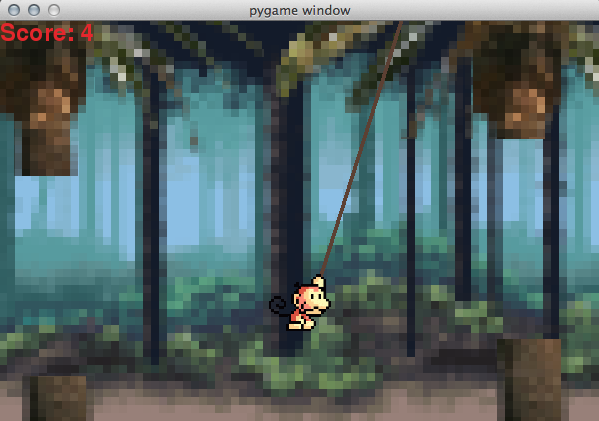
\includegraphics[width=0.49\textwidth]{figures/swingy}
        \label{fig:swingy}
    }\hfill
    \subfloat[SwingyMonkey State]{%
        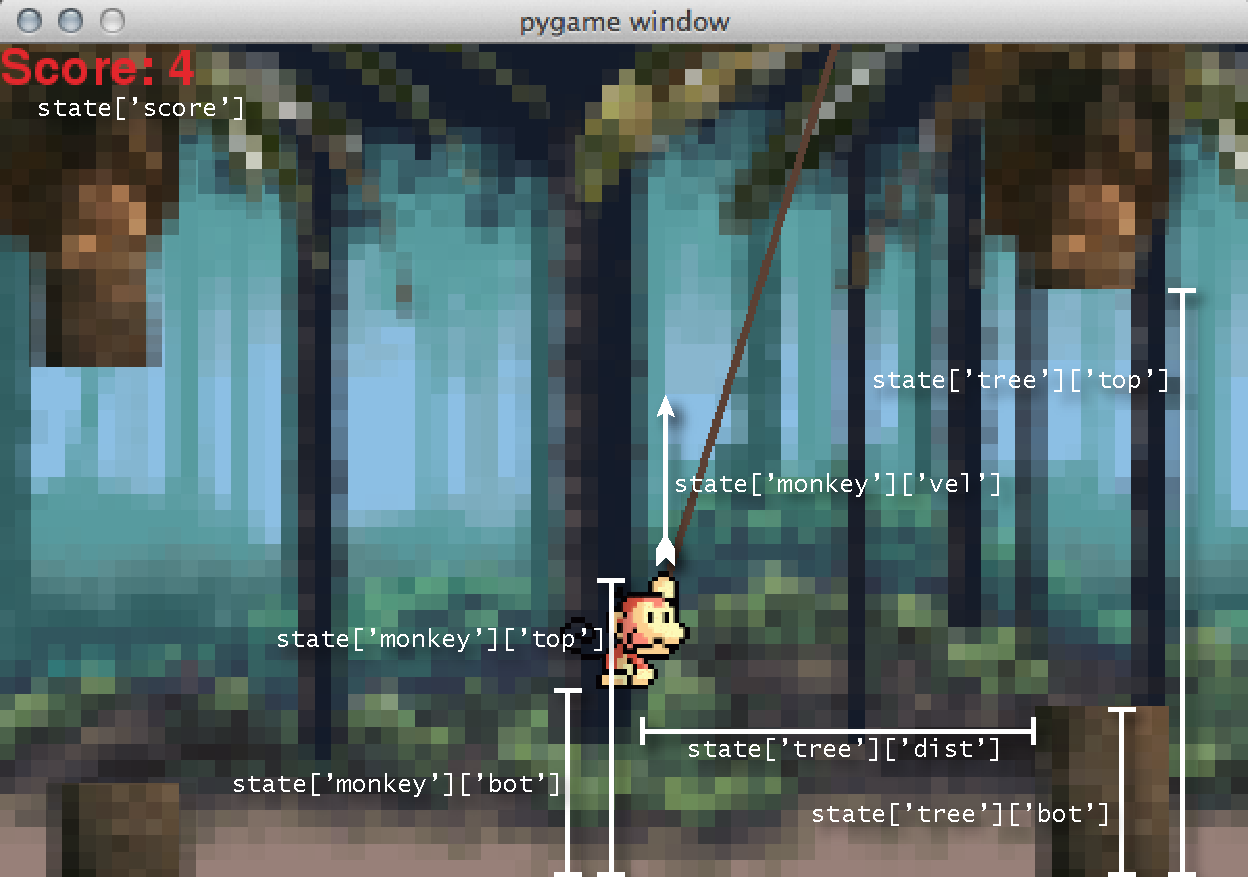
\includegraphics[width=0.49\textwidth]{figures/swingy-ann}
        \label{fig:swingy-ann}
    }
    \caption{(a) Screenshot of the Swingy Monkey game.  (b) Interpretations of various pieces of the state dictionary.}
\end{figure}

\section*{Evaluation}

Your task is to use reinforcement learning to find a policy for the monkey that can navigate the trees.  The implementation of the game itself is in file \verb|SwingyMonkey.py|, along with a few files in the \verb|res/| directory.  A file called \verb|stub.py| is provided to give you an idea of how you might go about setting up a learner that interacts with the game.  You can watch a YouTube video of the staff Q-Learner playing the game at \url{http://youtu.be/l4QjPr1uCac}.  You can see that it figures out a reasonable policy in a few dozen iterations.  You should explain how you decided to solve the problem, what decisions you made, and what issues you encountered along the way.  As in the other practicals, provide evidence where necessary to explain your decisions. You must have at least one plot or table that details the performances of different methods tried. For this practical, you'll need to use Python, as that's the language the game is written in. You should implement the MDP and reinforcement learning parts of this practical yourself. You should not use off-the-shelf RL tools to solve this, although you can use machine learning libraries.  {\bf Turn in your code!}




\end{document}